%--------------------------------------------%
% Template Beamer para Apresentações da UFRN %
% by alcemygvseverino@gmail.com              %
% Baseado em MIT Beamer Template			 %
% versao 1.1								 %
% Atualizado em 14/05/2016					 %
%--------------------------------------------%
%\documentclass[handout,t]{beamer}
\documentclass[presentation,t]{beamer}
% Para alterar a linguagem do documento
\usepackage[portuges]{babel}
% Para aceitar caracteres especias deretamente do teclado
\usepackage[utf8]{inputenc}
% Para seguir as normas da ABNT de citacao e referencias
\usepackage[alf]{abntex2cite}
% Para incluir figuras
\usepackage{graphicx}
% Para melhor ajuste da posisao das figuras
\usepackage{float}
% Para ajustar as dimensoes do layout da pagina
\usepackage{geometry}
% Para formatar estrutura e informacoes de formulas matematicas
\usepackage{amsmath}
% Para incluir simbolos especiais em formulas matematicas
\usepackage{amssymb}
% Para incluir links nas referencias
\usepackage{url}
% Para incluir paginas de documentos .pdf externos
\usepackage{pgfpages}
% Para ajustar o estilo dos contadores
\usepackage{enumerate}
% Para modificar a cor do texto
\usepackage{color}
% Para incluir condicoes
\usepackage{ifthen}
% Para colocar legendas em algo que nao e float
\usepackage{capt-of}
% Pacotes para escrever algoritmos em pseudocódigo
\usepackage[portuguese, ruled, linesnumbered]{algorithm2e}
% Para definir o tema do slide
\usetheme{Berlin}
% Para difinir cores e background
\usecolortheme{ufrn}
% Para numerar as figuras
\setbeamertemplate{caption}[numbered]

% Título
\title[DIM0117]{Estruturas de Dados Básicas II}
% Data
\date{\today}
% Autores
\author[Valdigleis]{Valdigleis\inst{1}}
	%\vspace{0.25cm}
	%Autor 02 \inst{2}
%}

% Instituto
\institute[UFRN]{
	\inst{1}%
        Universidade Federal do Rio Grande do Norte\\
        Centro de Ciência Exatas e da Terra\\
        Departamento de Informática e Matemática Aplicada\\
	\url{valdigleis@dimap.ufrn.br}\\
	\vspace{0.25cm}
	%\inst{2}%
	%Departamento\\
}

% Logo do canto inferior direito
\pgfdeclareimage[height=0.7cm]{logo_UFRN}{figuras/logo_UFRN}
\logo{\vspace*{-0.25cm}\pgfuseimage{logo_UFRN}\hspace*{-0.05cm}}


\begin{document}
% Sumário
\frame{\titlepage}
\section[]{}
\begin{frame}{Sumário}
	\tableofcontents
\end{frame}

% seções
\section{Fundamentação de POO}

\begin{frame}{Relembrando o paradigma procedural}
  \begin{itemize}
    \item É baseado no conceito de chamada de funções por um fluxo de dados.
    \item Todas as variáveis são concentradas no fluxo de dados.
    \item As funções tomam um conjunto de variáveis como argumento e retorna o resultado para o fluxo de dados.
  \end{itemize}
  \begin{figure}
    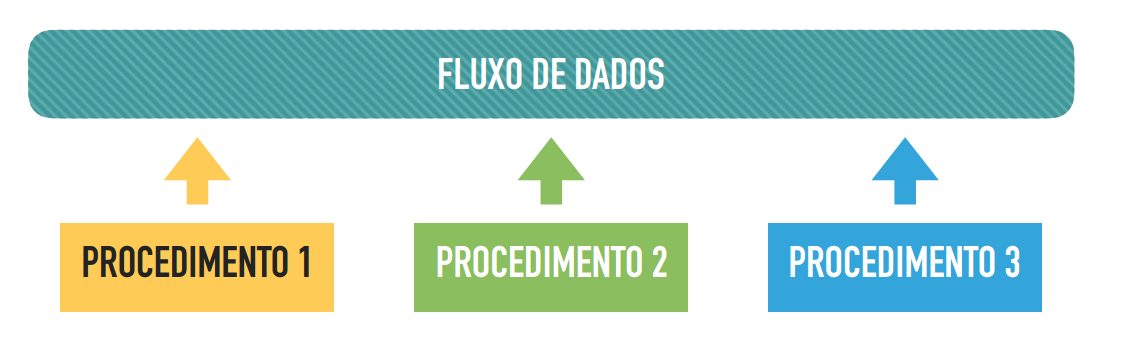
\includegraphics[width=0.85\textwidth]{figuras/fluxo.png}
    \caption{Estrutura do padadigma procedural.}
  \end{figure}
\end{frame}

\begin{frame}{Clases x Objetos}
  \begin{itemize}
    \item Uma classe é o molde especificando quais atributos (dados) e métodos (funções) os objetos criados a partir dela terão.\pause
    \item Um objeto é uma instância de uma classe, ou seja, é um individo criado a partir do molde em que é possível obter o \textbf{estado} de seus atributos. Sobre os métodos, eles são as ações que um objeto pode realizar.
  \end{itemize}
  \pause
  {\color{red}Importante}: Sobre os objetos, eles apresentam a ideia de \textbf{ciclo de vida}, eles podem ser (1) criados, (2) manipulados e (3) destruídos.
\end{frame}

\begin{frame}{O que é o paradigma OO?}
  \begin{itemize}
    \item Paradigma para desenvolvimento de software que baseia-se na noção de utilização de componentes individuais e simples (os objetos) e na comunicação (troca de mensagens) entre esse componentes para construir sistemas mais complexos.
  \end{itemize}
  \pause
  E quais as vantagens de OO?
  \begin{itemize}
    \item Facilita para reutilizar código (não reinventar a roda).
    \item A modelagem é ligeiramente aproximada, com a realidade do mundo.
    \item Pequenas mudanças nos requisitos dos sistemas não tem grandes impactos no desenvolvimento.
  \end{itemize}
\end{frame}
\section{Os quatro pilares de OO}

\begin{frame}{Os pilares}
  \begin{itemize}
    \item Abstração: são as classes propriamente ditas, elas são definidas em termos de código e são fundamentais pois define os objetos no sistema.\pause
    \item Encapsulamento: refere-se à prática de restringir o acesso direto aos atributos e métodos internos de um objeto, permitindo o controle desse acesso por meio de métodos específicos.\pause
    \item Herança: permite a criação de novas classes a partir de classes existentes, reutilizando atributos e métodos. Isso promove a reutilização de código e facilita a manutenção.\pause
    \item Polimorfismo: permite que os métodos tenham comportamentos diferentes dependendo do objeto que os invoca ou do contexto em que são utilizados.
  \end{itemize}
\end{frame}

\begin{frame}{Sobre o Encapsulamento}
  O Encapsulamento tem por objetivos:
  \begin{itemize}
    \item Proteção dos dados, ou seja, vita modificações acidentais ou indevidas do estado dos objetos.
    \item Esconder a implementação, o usuário da classe interage apenas com a interface ``pública'', sem precisar conhecer os detalhes internos.
    \item Facilitar a manutenção, isto é, alterações na implementação não devem afetar quem usa a classe.
  \end{itemize}
  \pause
  E quais o níveis de proteção dos dados?\pause O níveis são: privado, protegido e público.
\end{frame}

\begin{frame}{Sobre Herança}
  As heranças podem ser
  \begin{itemize}
    \item Herança Simples: Uma subclasse herda de uma única superclasse. (Java e PHP seguem esse modelo).
    \item Herança Múltipla: Uma classe herda de múltiplas classes (existe em Python, C++, mas não existe em Java).
    \item Herança Multinível (encadeada): Uma classe herda de outra que já herdou de uma terceira.
    \item Herança Hierárquica: Uma superclasse tem várias subclasses.
  \end{itemize}
\end{frame}

\begin{frame}{Sobre Polimorfismo}
  O Polimorfismo tem por objetos:
  \begin{itemize}
    \item Flexibilidade: Permite que um mesmo método ou interface seja usado para diferentes tipos de objetos.
    \item Extensibilidade: Facilita a adição de novos tipos de objetos sem modificar o código existente.
    \item Abstração: Permite trabalhar com objetos de forma genérica, sem precisar conhecer seus tipos específicos.
  \end{itemize}
  \pause
  Como o polimorfismo é implementado?\pause
  \begin{itemize}
    \item Sobrescrita de métodos (override): Uma classe filha redefine um método da classe pai.
    \item Sobrecarga de métodos (overload): vários métodos com o mesmo nome, mas com parâmetros diferentes.
    \item Interfaces e classes abstratas, definem métodos que devem ser implementados pelas classes filhas.
  \end{itemize}
\end{frame}
\section{Como representar algoritmos?}

\begin{frame}{Formas de representação}
  Existem no mínimo duas formas bem difundidas de como representar algoritmos: \textbf{Linguagem natural}, \textbf{Fluxograma} e \textbf{Pseudocódigo}.
  \begin{itemize}
    \item \textbf{Linguagem natural}: o Algoritmo é escrito em frases comuns, como uma explicação passo a passo. Por exemplo, \textit{\color{blue}Para encontrar o maior número em uma lista, percorra cada elemento e compare com o maior já encontrado. Se for maior, atualize. No final, o maior número será o resultado.}.
  \end{itemize}
\end{frame}

\begin{frame}{Formas de representação}
  Existem no mínimo duas formas bem difundidas de como representar algoritmos: \textbf{Linguagem natural}, \textbf{Fluxograma} e \textbf{Pseudocódigo}.
  \begin{itemize}
    \item \textbf{Fluxograma}: os algoritmos são representados de forma visual usando diagramas que representam o fluxo de execução do algoritmo.
  \end{itemize}
  \begin{figure}
    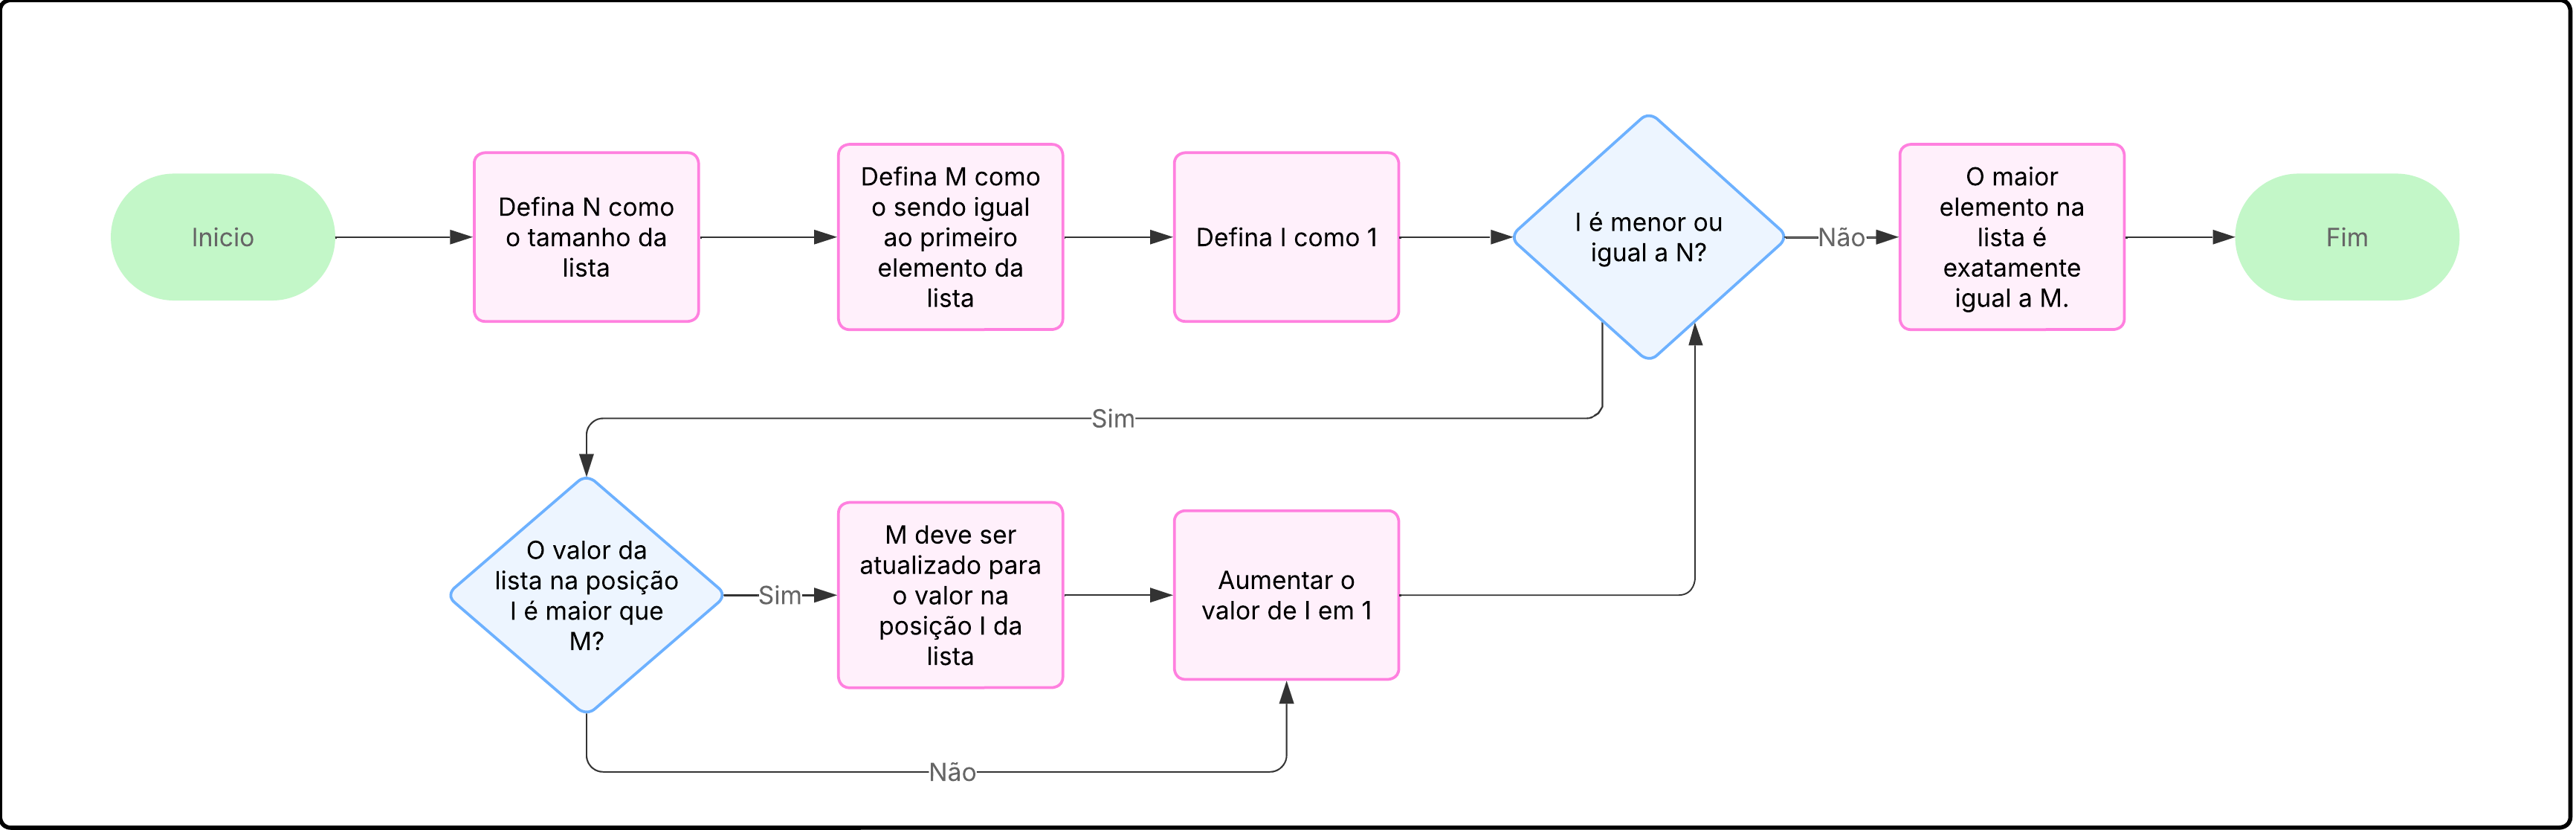
\includegraphics[width=0.85\textwidth]{figuras/Fluxograma}
  \end{figure}
\end{frame}

\begin{frame}{Sobre os fluxogramas}
  Os símbolos padronizados usados no fluxograma podem ser compreendidos da seguinte forma:
  \begin{enumerate}
    \item Elipse: indica o ponto inicial e o ponto final do fluxograma.
    \item Retângulo: representa uma operação ou ação, como calcular, armazenar um valor ou executar uma tarefa.
    \item Paralelogramo: indica operações de entrada (como receber dados do usuário) e saída (mostrar um resultado).
    \item Losango: representa um ponto onde o fluxo pode seguir diferentes direções, dependendo de uma condição lógica.
  \end{enumerate}
\end{frame}

\begin{frame}{Formas de representação}
  Existem no mínimo duas formas bem difundidas de como representar algoritmos: \textbf{Linguagem natural}, \textbf{Fluxograma} e \textbf{Pseudocódigo}.
  \begin{itemize}
    \item \textbf{Pseudocódigo}:  é uma forma estruturada de representar algoritmos utilizando uma mistura de linguagem natural e elementos de linguagens de programação.
  \end{itemize}
\end{frame}

\begin{frame}{Exemplo de Pseudocódigo}
  \begin{algorithm}[H]
    \SetAlgoLined
    \Entrada{A lista $L$ de tamanho $N$} 
    \Saida{O maior valor em $L$}
    \Inicio{
      $i = 1$\\
      $M = L[0]$\\
      \Enqto{$i < N$}{
        \Se{$L[i] > M$}{
          $M = L[i]$\\
        }
      }
    }
    \Retorna{$M$}
    \label{alg1}
    \caption{Algoritmo para encontrar o maior valor na lista.}
  \end{algorithm}
\end{frame}



\begin{frame}{Referências}
  \bibliography{referencias}
\end{frame}

\end{document}
